% Options for packages loaded elsewhere
\PassOptionsToPackage{unicode}{hyperref}
\PassOptionsToPackage{hyphens}{url}
%
\documentclass[
  english,
  man]{apa6}
\usepackage{lmodern}
\usepackage{amssymb,amsmath}
\usepackage{ifxetex,ifluatex}
\ifnum 0\ifxetex 1\fi\ifluatex 1\fi=0 % if pdftex
  \usepackage[T1]{fontenc}
  \usepackage[utf8]{inputenc}
  \usepackage{textcomp} % provide euro and other symbols
\else % if luatex or xetex
  \usepackage{unicode-math}
  \defaultfontfeatures{Scale=MatchLowercase}
  \defaultfontfeatures[\rmfamily]{Ligatures=TeX,Scale=1}
\fi
% Use upquote if available, for straight quotes in verbatim environments
\IfFileExists{upquote.sty}{\usepackage{upquote}}{}
\IfFileExists{microtype.sty}{% use microtype if available
  \usepackage[]{microtype}
  \UseMicrotypeSet[protrusion]{basicmath} % disable protrusion for tt fonts
}{}
\makeatletter
\@ifundefined{KOMAClassName}{% if non-KOMA class
  \IfFileExists{parskip.sty}{%
    \usepackage{parskip}
  }{% else
    \setlength{\parindent}{0pt}
    \setlength{\parskip}{6pt plus 2pt minus 1pt}}
}{% if KOMA class
  \KOMAoptions{parskip=half}}
\makeatother
\usepackage{xcolor}
\IfFileExists{xurl.sty}{\usepackage{xurl}}{} % add URL line breaks if available
\IfFileExists{bookmark.sty}{\usepackage{bookmark}}{\usepackage{hyperref}}
\hypersetup{
  pdftitle={Surprise! Low Testing Expectancy Moderates the Sans Forgetica Effect},
  pdfauthor={Jason Geller1,2},
  pdflang={en-EN},
  pdfkeywords={Disfluency},
  hidelinks,
  pdfcreator={LaTeX via pandoc}}
\urlstyle{same} % disable monospaced font for URLs
\usepackage{graphicx,grffile}
\makeatletter
\def\maxwidth{\ifdim\Gin@nat@width>\linewidth\linewidth\else\Gin@nat@width\fi}
\def\maxheight{\ifdim\Gin@nat@height>\textheight\textheight\else\Gin@nat@height\fi}
\makeatother
% Scale images if necessary, so that they will not overflow the page
% margins by default, and it is still possible to overwrite the defaults
% using explicit options in \includegraphics[width, height, ...]{}
\setkeys{Gin}{width=\maxwidth,height=\maxheight,keepaspectratio}
% Set default figure placement to htbp
\makeatletter
\def\fps@figure{htbp}
\makeatother
\setlength{\emergencystretch}{3em} % prevent overfull lines
\providecommand{\tightlist}{%
  \setlength{\itemsep}{0pt}\setlength{\parskip}{0pt}}
\setcounter{secnumdepth}{-\maxdimen} % remove section numbering
% Make \paragraph and \subparagraph free-standing
\ifx\paragraph\undefined\else
  \let\oldparagraph\paragraph
  \renewcommand{\paragraph}[1]{\oldparagraph{#1}\mbox{}}
\fi
\ifx\subparagraph\undefined\else
  \let\oldsubparagraph\subparagraph
  \renewcommand{\subparagraph}[1]{\oldsubparagraph{#1}\mbox{}}
\fi
% Manuscript styling
\usepackage{upgreek}
\captionsetup{font=singlespacing,justification=justified}

% Table formatting
\usepackage{longtable}
\usepackage{lscape}
% \usepackage[counterclockwise]{rotating}   % Landscape page setup for large tables
\usepackage{multirow}		% Table styling
\usepackage{tabularx}		% Control Column width
\usepackage[flushleft]{threeparttable}	% Allows for three part tables with a specified notes section
\usepackage{threeparttablex}            % Lets threeparttable work with longtable

% Create new environments so endfloat can handle them
% \newenvironment{ltable}
%   {\begin{landscape}\begin{center}\begin{threeparttable}}
%   {\end{threeparttable}\end{center}\end{landscape}}
\newenvironment{lltable}{\begin{landscape}\begin{center}\begin{ThreePartTable}}{\end{ThreePartTable}\end{center}\end{landscape}}

% Enables adjusting longtable caption width to table width
% Solution found at http://golatex.de/longtable-mit-caption-so-breit-wie-die-tabelle-t15767.html
\makeatletter
\newcommand\LastLTentrywidth{1em}
\newlength\longtablewidth
\setlength{\longtablewidth}{1in}
\newcommand{\getlongtablewidth}{\begingroup \ifcsname LT@\roman{LT@tables}\endcsname \global\longtablewidth=0pt \renewcommand{\LT@entry}[2]{\global\advance\longtablewidth by ##2\relax\gdef\LastLTentrywidth{##2}}\@nameuse{LT@\roman{LT@tables}} \fi \endgroup}

% \setlength{\parindent}{0.5in}
% \setlength{\parskip}{0pt plus 0pt minus 0pt}

% \usepackage{etoolbox}
\makeatletter
\patchcmd{\HyOrg@maketitle}
  {\section{\normalfont\normalsize\abstractname}}
  {\section*{\normalfont\normalsize\abstractname}}
  {}{\typeout{Failed to patch abstract.}}
\patchcmd{\HyOrg@maketitle}
  {\section{\protect\normalfont{\@title}}}
  {\section*{\protect\normalfont{\@title}}}
  {}{\typeout{Failed to patch title.}}
\makeatother
\shorttitle{SHORTTITLE}
\keywords{Disfluency\newline\indent Word count: X}
\DeclareDelayedFloatFlavor{ThreePartTable}{table}
\DeclareDelayedFloatFlavor{lltable}{table}
\DeclareDelayedFloatFlavor*{longtable}{table}
\makeatletter
\renewcommand{\efloat@iwrite}[1]{\immediate\expandafter\protected@write\csname efloat@post#1\endcsname{}}
\makeatother
\usepackage{lineno}

\linenumbers
\usepackage{csquotes}
\ifxetex
  % Load polyglossia as late as possible: uses bidi with RTL langages (e.g. Hebrew, Arabic)
  \usepackage{polyglossia}
  \setmainlanguage[]{english}
\else
  \usepackage[shorthands=off,main=english]{babel}
\fi

\title{Surprise! Low Testing Expectancy Moderates the Sans Forgetica Effect}
\author{Jason Geller\textsuperscript{1,2}}
\date{}


\authornote{

Add complete departmental affiliations for each author here. Each new line herein must be indented, like this line.

Enter author note here.

Correspondence concerning this article should be addressed to Jason Geller, Rutgers University Center for Cognitive Science (RuCCS), 152 Frelinghuysen Road, Busch Campus, Piscataway, New Jersey 08854. E-mail: \href{mailto:jason.geller@ruccs.rutgers.edu}{\nolinkurl{jason.geller@ruccs.rutgers.edu}}

}

\affiliation{\vspace{0.5cm}\textsuperscript{1} University of Iowa\\\textsuperscript{2} Rutgers University Center for Cognitive Science}

\abstract{
Recent work examaining Sans Forgetica have shown both postive, negative, and null mnenmonic effects. A possible explanation for the mixed evidence is the study design employed. Studies failing to show a positive Sans Forgetica effect have told particiapnts about an upcoming test (high testing expectancy). This could have the unintenital consequence of countervailing any postive effect exerted by Sans Forgetica by engendering deeper processing for all studied material. To test this, we conduced two experiments using a yes/no recognition memory test (Experiment 1) and a cued recall test (Experiment 2). In Experiment 1, Sans Forgetica overall eliciated lower judgements of learning and longer study times, but Sans Forgetica only improved improved memory when there was low test expectancy (compared to high test expectancy). In Experiment 2, using only a low test expectancy design, we found a similar pattern of results. That is, Sans Forgetia elictsed lower JOLs and longer study times, and produced better cued memory recall. Herein we have shown a boundary condition for the Sans Forgetica effect. Caution should be taken, however. The finding that Sans forgetica only occurs under low expectancy delimits its utility as an effective study tool. Those wanting to remember more and forget less should stick to other desirable difficultues proven to enhance memory.
}



\begin{document}
\maketitle

The influential desirable difficulty principle suggests that making learning harder not easier, such as having students take a test over information previously studied, can have noticeable and lasting impacts on student achievement (Bjork \& Bjork, 2011; see Sotola \& Crede, 2020 for a recent meta-analysis). Recently, the concept of desirable difficulties has been extended to include subtle perceptual manipulations that are difficult to encode (e.g., atypical fonts, blurring, handwritten cursive; {\textbf{???}}; {\textbf{???}}; Geller et al., 2018). One such perceptual disfluency manipulation garnering increased attention from news outlets (NPR and Washington Post) and researchers alike is the Sans Forgetica typeface. Sans Forgetica is a typeface developed by a team of psychologists, graphic designers, and marketers, consisting of intermittent gaps and black-slanted letters ({\textbf{???}}). The disfluent perceptual characteristics of Sans Forgetica are purported to stave off forgetting and enhance learning. However, as the famous astronomer Carl Sagan once said, "Extraordinary claims require extraordinary evidence (Sagan, 1980).

In two independent attempts, Taylor, Sanson, Burnell, Wade, and Garry (2020) and Geller, Davis, and Peterson (2020) set out to examine whether Sans Forgetica is \emph{really} a desirable difficulty. In the first conceptual replications of the Sans Forgetica effect, Taylor et al. (2020), found (in a sample of 882 people across 4 experiments) that while Sans Forgetica was perceived as more disfluent by participants (Experiment 1) there was no evidence that Sans Forgetica yielded a mnemonic boost in cued recall with highly related word pairs (Experiment 2) compared to a fluent typeface (Arial) or when learning simple prose passages (Experiments 3-4). Extending these findings, Geller et al. (2020) conducted three pre-registered experiments with over 800 participants, and found, similar to ({\textbf{???}}), that Sans Forgetica does not enhance learning for weakly related word pairs (Experiment 1), a complex prose passage on ground water (Experiment 2), or when the type of test was changed to a recognition memory test (Experiment 3). Taken together, across two independent replication attempts, and over a 1000 participants, there is weak evidence for a Sans Forgetica memory effect.

Despite these findings, some evidence for the effectiveness of the Sans Forgetica typeface does exist. For instance, Eskenazi and Nix (2020) found that Sans Forgetica can enhance learning. Using eye-tracking, Eskenazi and Nix (2020) had participants learn the spelling and meaning for 15 low-frequency words each presented in the context of two sentences. Both orthographic discriminabity (i.e., choosing the correct spelling of a word) and semantic acquisition (i.e., retrieving the definition of a word) were assessed. The authors reported a memory benefit for both orthographic discrimnability and semantics for words presented in Sans Forgetica compared to a normal (Courier) typeface, but only for participants that were good spellers.

The mixed findings suggest that the Sans Forgetica may be fickle, with positive effects potentially bounded by specific conditions. Probing into Eskenazi and Nix (2020), a critical difference between their study and ({\textbf{???}}) and Geller et al. (2020), is testing expectancy. That is, in Eskenazi and Nix (2020), they did did not tell their participants about the upcoming tests. Thus, one common design feature that may moderate whether we see a Sans Forgetica effect is high testing expectancy. Eitel and Kühl (2016) posited that testing expectancy may be an important moderator of the perceptual disfluency effect. They reasoned that if the disfluency effect arises because of deeper, more effortful, processing, telling participants about a memory test should eliminate the effect. This occurs because testing expectancy would countervail the effects of perceptual disfluency by eliciting additional processing for both fluent and disfluent stimuli. In contrast, low testing expectancy is less likely to impact processing of individual items,leaving effects of processing difficulty intact. While Eitel and Kühl (2016) did not find evidence for this,Geller and Still (2018), using a masking disfluency manipulation, demonstrated in a yes/no recognition memory test that indeed only under low testing expectancy does a disfluency effect occur. Given this, it is possible, then, that a Sans Forgetica effect might arise when participants have low test expectancy.

\hypertarget{experiment-1}{%
\section{Experiment 1}\label{experiment-1}}

Experiment 1 examined whether the positive effects of Sans Forgetica (as seen in Eskenazi \& Nix, 2020) were moderated by testing expectancy. Using a yes/no recognition memory test, we manipulated whether individuals were told about an upcoming memory test. In addition, we examined participants study times and judgments of learning (JOLs) to Sans Forgetica stimuli. We preregistered that the Sans Forgetica effect would be moderated by testing expectancy insofar when participants were not told about a memory test we would see effect, but not if they were told about a memory test. I predicted that\ldots{}

\hypertarget{method}{%
\section{Method}\label{method}}

Sample size, experimental design, hypotheses, outcome measures, and analysis plan for Experiment 1 were can be found on the Open Science Framework (\url{https://osf.io/wgp9d}). All raw and summary data, materials, and R scripts for pre-processing, analysis, and plotting can be found at \url{https://osf.io/d2vy8/}.

\hypertarget{participants}{%
\subsection{Participants}\label{participants}}

We preregistered a sample size of 230. All participants were recruited through prolific (prolific.co), and completed the study on the Gorilla platform {[}www.gorilla.sc; Anwyl-Irvine2020{]}. The sample size was based off a previous experiment (Geller et al. (2020), Experiment 1), wherein they calculated power to detect a medium sized interaction effect (\emph{d} = 0.35) using a similar design to the current study. After data collection had ended we had a total of 231 participants. Participants completed the experiment in return for U.S.\$8.00 an hour.

\hypertarget{materials}{%
\subsubsection{Materials}\label{materials}}

Stimuli were 188 single-word nouns taken from Geller et al.~(2018). All words were from the English Lexicon Project database (Balota et al., 2007). Both word frequency (all words were high frequency; mean log HAL frequency = 9.2) and length (all words were four letters) were controlled. The full set of stimuli can be found at \url{https://osf.io/dsxrc/}.

\hypertarget{design}{%
\subsubsection{Design}\label{design}}

Per our pre-registration, d', JOLs, and study times were analyzed with a 2 (Typeface: Arial vs.~Sans Forgetica ) x 2 (Testing Expectancy: High vs.~Low) mixed analysis of variance (ANOVA).

\hypertarget{procedure}{%
\subsubsection{Procedure}\label{procedure}}

Similar to Geller et al. (2020) (Experiment 3), we presented all participants with 188 words, 94 at study (47 in each typeface condition) and 188 at test (94 old and 94 new). Words were counterbalanced across the typeface and study/test conditions, such that each word served equally often as a target and a foil in both typefaces across participants. This lead to the creation of 4 counterbalanced lists. Word order was completely randomized, such that Arial and Sans Forgetica words were randomly intermixed in the study phase, and Arial and Sans Forgetica old and new words were randomly intermixed in the test phase, with old words always presented in the same typeface at test as they were at study.

The main difference between the current experiment and Geller et al. (2020) (Experiment 3) is that participants were randomly assigned to one of two conditions: the high expectancy test condition or the low expectancy test condition. Interested readers can view the entire task including insturctions for each condition by following these links () ().

The experiment proper consisted of four phases: a study phase,JOL phase, distractor phase, and test phase. During the study phase, a fixation cross appeared at the center of the screen for 500 ms. The fixation cross was immediately replaced by a word in the same location. To continue to the next trial, participants pressed the continue button at the bottom of the screen. Each trial was self-paced. After the study phase, participants completed a short three-minute distractor task wherein they wrote down as many U.S. state capitals as they could. Afterward, participants took an old-new recognition test. During the test phase, a word appeared in the center of the screen that either had been presented during study (\enquote{old}) or had not been presented during study (\enquote{new}). Old words occurred in their original typeface, and following the counterbalancing procedure, each new word was presented in Arial typeface or Sans Forgetica typeface. For each word presented, participants chose from one of two boxes displayed on the screen: a box labeled \enquote{old} to indicate that they had studied the word during study, and a box labeled \enquote{new} to indicate they did not remember studying the word. Sans Forgetica Words stayed on the screen until participants gave an \enquote{old} or \enquote{new} response. All words were individually randomized for each participant during both the study and test phases. After the experiment, participants were debriefed.

\hypertarget{analytic-strategy}{%
\subsubsection{Analytic Strategy}\label{analytic-strategy}}

For both experiments, an alpha level of .05 is maintained. Cohen's \emph{d} and generalized eta-squared (\(\eta_{g}^{2}\)\}; {\textbf{???}}) are used as effect size measures. Alongside traditional analyses that utilize null hypothesis significance testing (NHST), we also report the Bayes factors (BFs) for reported null effects. A Bayes Factor \textgreater{} = 3 will be deemed as moderate evidence for null; BF \textgreater{} =10 strong evidence for the null. All data were analyzed in R (vers. 4.0.2; R Core Team, 2020), with models fit using the afex (vers. 0.27-2; Singmann, Bolker, Westfall, Aust, and Ben-Shachar (2020)) and BayesFactor packages (vers. 0.9.12-4.2; Morey and Rouder (2018)). All figures were generated using ggplot2 (vers. 3.3.0; Wickham, 2006).

\hypertarget{results-and-discussion}{%
\subsection{Results and Discussion}\label{results-and-discussion}}

\hypertarget{recognition-memory}{%
\subsubsection{Recognition Memory}\label{recognition-memory}}

Performance was examined with d', a memory sensitivity measure derived from signal detection theory (Macmillan \& Creelman, 2005). Hits or false alarms at ceiling or floor were changed to .99 or .01. Hits and false alarms along with sensitivity (d') can be seen in Figure 1. Participants that were told about a memory test performed better (\emph{M} = 0.88) than those not told about a memory test (\emph{M} = .72),\emph{M} \textsubscript{diff} = 0.16,\emph{F}(1, 229) = 4.11, \(\eta_{g}^{2}\) = .014, p = .044. Individuals were better at discriminating target words presented in Sans Forgetica (\emph{M} = .86) than Arial (\emph{M} = .74) ,\emph{M} \textsubscript{diff} = .12, \emph{F}(1, 229) = 10.73, \(\eta_{g}^{2}\) =.010, \emph{p} = .001. This was qualified by an interaction between Test Expectancy and Typeface, \emph{F}(1, 229) = 4.34, \(\eta_{g}^{2}\) = .004, \emph{p} = .038. Simple effects showed that individuals in the low expectancy group showed better recognition memory for words presented in Sans Forgetica font compared to Arial, \emph{F}(1, 229) = 14.297, \emph{p} \textless{} .001, \emph{d} = 0.31. In the high test expectancy group, there was d` differences between the two typefaces, \emph{F}(1, 229) = 0.716, \emph{p} = .398, BF\textsubscript{O1} = 5.83.

\#High Testing Data Load

\begin{verbatim}
## Warning in require_bit64_if_needed(ans): Some columns are type 'integer64'
## but package bit64 is not installed. Those columns will print as strange
## looking floating point data. There is no need to reload the data. Simply
## install.packages('bit64') to obtain the integer64 print method and print the
## data again.

## Warning in require_bit64_if_needed(ans): Some columns are type 'integer64'
## but package bit64 is not installed. Those columns will print as strange
## looking floating point data. There is no need to reload the data. Simply
## install.packages('bit64') to obtain the integer64 print method and print the
## data again.

## Warning in require_bit64_if_needed(ans): Some columns are type 'integer64'
## but package bit64 is not installed. Those columns will print as strange
## looking floating point data. There is no need to reload the data. Simply
## install.packages('bit64') to obtain the integer64 print method and print the
## data again.

## Warning in require_bit64_if_needed(ans): Some columns are type 'integer64'
## but package bit64 is not installed. Those columns will print as strange
## looking floating point data. There is no need to reload the data. Simply
## install.packages('bit64') to obtain the integer64 print method and print the
## data again.
\end{verbatim}

\#Combine

\begin{verbatim}
## # A tibble: 462 x 11
##    participant_pri~ condition1 testexpect    cr    fa   hit  miss    hr     zhr
##               <int> <chr>      <chr>      <int> <dbl> <int> <int> <dbl>   <dbl>
##  1          1531474 Arial      low           37 0.213    21    26 0.447 -0.134 
##  2          1531474 Sans Forg~ low           36 0.234    20    27 0.426 -0.188 
##  3          1531487 Arial      low           25 0.468    20    27 0.426 -0.188 
##  4          1531487 Sans Forg~ low           26 0.447    23    24 0.489 -0.0267
##  5          1531488 Arial      low           40 0.149    20    27 0.426 -0.188 
##  6          1531488 Sans Forg~ low           34 0.277    32    15 0.681  0.470 
##  7          1531494 Arial      low           47 0.01     42     5 0.894  1.25  
##  8          1531494 Sans Forg~ low           47 0.01     42     5 0.894  1.25  
##  9          1531503 Arial      low           30 0.362    18    29 0.383 -0.298 
## 10          1531503 Sans Forg~ low           12 0.745    32    15 0.681  0.470 
## # ... with 452 more rows, and 2 more variables: zfa <dbl>, dprime <dbl>
\end{verbatim}

\begin{verbatim}
## 
## Univariate Type III Repeated-Measures ANOVA Assuming Sphericity
## 
##                        Sum Sq num Df Error SS den Df  F value    Pr(>F)    
## (Intercept)           296.652      1  166.184    229 408.7834 < 2.2e-16 ***
## testexpect              2.980      1  166.184    229   4.1058  0.043896 *  
## condition1              1.818      1   38.786    229  10.7344  0.001215 ** 
## testexpect:condition1   0.735      1   38.786    229   4.3369  0.038405 *  
## ---
## Signif. codes:  0 '***' 0.001 '**' 0.01 '*' 0.05 '.' 0.1 ' ' 1
\end{verbatim}

\begin{verbatim}
## Anova Table (Type 3 tests)
## 
## Response: dprime
##                  Effect     df  MSE        F  ges p.value
## 1            testexpect 1, 229 0.73   4.11 * .014    .044
## 2            condition1 1, 229 0.17 10.73 ** .009    .001
## 3 testexpect:condition1 1, 229 0.17   4.34 * .004    .038
## ---
## Signif. codes:  0 '***' 0.001 '**' 0.01 '*' 0.05 '+' 0.1 ' ' 1
\end{verbatim}

\hypertarget{jols}{%
\subsubsection{JOLs}\label{jols}}

Seven participants were removed for either not providing JOls to each typeface, or only providing one response. Using the same model as above, JOLs were higher when testing expectancy was lower, \emph{F}(1,221) = 16.01, \(\eta_{g}^{2}\) = .065, \emph{p} \textless{} .001. JOLs were lower for Sans Forgetica (\emph{M} = 57.5) compared to Arial (\emph{M} = 61.5), \emph{M} \textsubscript{diff} = 4.0, \emph{F}(1,221) = 27.05, \(\eta_{g}^{2}\) = .004, \emph{p} \textless{} .001. There was no interaction between Testing Expectancy and Typeface, \emph{F}(1,221) = 0.13, \(\eta_{g}^{2}\) \textless{} .001, \emph{P} = .715.There was little evidence for an interaction, BF\textsubscript{01} = 7.28.

\hypertarget{study-times}{%
\subsubsection{Study Times}\label{study-times}}

Although not pre-registered, we excluded reaction times less than 200 ms and reaction times greater than 2.5 SD above the mean per condition for each participant. The outlier procedure removed \textasciitilde3 \% of the data. Given reactions times are notoriously positively skewed, we also log transformed the data (see Fig.1C for reaction time data). Testing Expectancy did not influence reading times, \emph{F}(1,229) = 1.97, \(\eta_{g}^{2}\) = .008, \emph{p} = .162, BF. Typeface did influence reading times. Response latencies were overall slower for Sans Forgetica than Arial, \emph{F}(1,229) = 30.91, \(\eta_{g}^{2}\) = .001, \emph{p} \textless{} .001. There was no interaction between Testing Expectancy and Typeface, \emph{F}(1,229) = 1.10, \(\eta_{g}^{2}\) \textless{} .001, \emph{p} = .296.

\begin{verbatim}
## 
## Univariate Type III Repeated-Measures ANOVA Assuming Sphericity
## 
##                     Sum Sq num Df Error SS den Df    F value    Pr(>F)    
## (Intercept)        20706.2      1  168.431    229 28152.2648 < 2.2e-16 ***
## testexpt               1.1      1  168.431    229     1.5354    0.2166    
## condition              0.3      1    1.797    229    33.0251 2.884e-08 ***
## testexpt:condition     0.0      1    1.797    229     1.1292    0.2891    
## ---
## Signif. codes:  0 '***' 0.001 '**' 0.01 '*' 0.05 '.' 0.1 ' ' 1
\end{verbatim}

\begin{figure}

{\centering 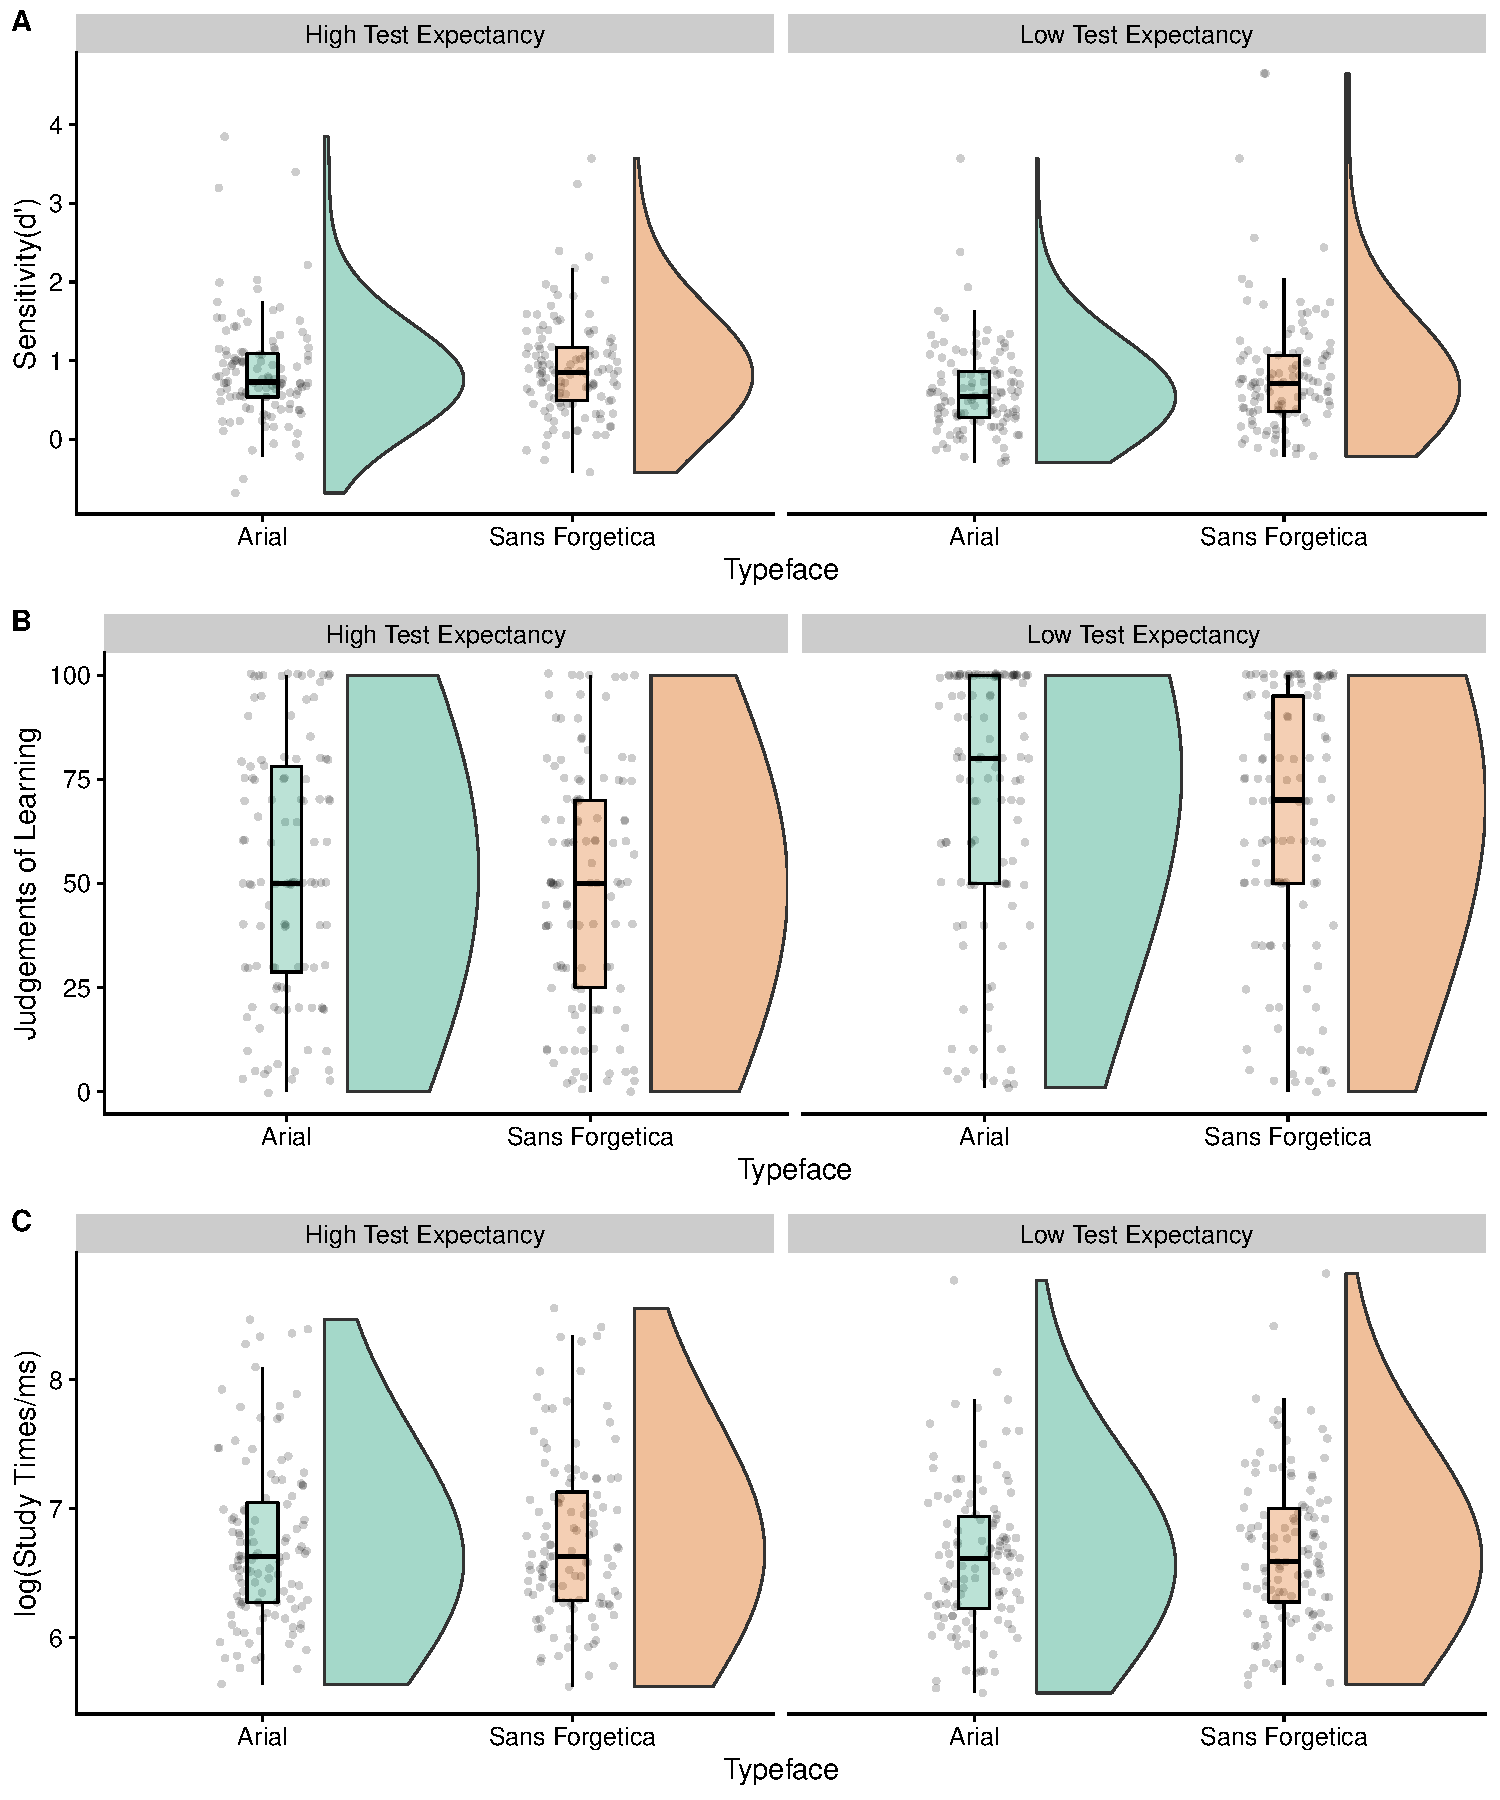
\includegraphics{Testing_Expectancy_SF_files/figure-latex/unnamed-chunk-15-1} 

}

\caption{Raincloud plots (Allen et al., 2019) depicting raw data (dots), box plots, and half violin kernel desntiy plots.A.Memory sensitivity (d') as a function of Typeface and Testing Expectancy. B. Judgements of Learning as a function of Typeface and Test Expectany. C. Study times (log transformed) as a function of Typeface and Test Expextancy. Raincloud plots (Allen et al., 2019) depicting raw data (dots), box plots, and half violin kernelViolin plots represent the kernal density of avearge accuracy (black dots) with the mean (white dot)}\label{fig:unnamed-chunk-15}
\end{figure}

\hypertarget{experiment-2}{%
\section{Experiment 2}\label{experiment-2}}

\hypertarget{methods}{%
\subsection{Methods}\label{methods}}

\hypertarget{participants-1}{%
\subsubsection{Participants}\label{participants-1}}

One hundred and sixteen participants (\emph{N} = 116) participated through Prolific for U.S. \$2.43. All participants were native English speakers with normal or corrected-to-normal vision. A sensitivity analysis conducted with the R package pwr(Champely, 2020) indicated that our sample size provided 90\% power to detect a small effect size (d = 0.16) or larger.

\hypertarget{design-1}{%
\subsubsection{Design}\label{design-1}}

We examined cued recall accuracy, JOLs, and reading times to Typefaces (Sans Forgetica vs.~Arial) with a paired \emph{t}-test.

\hypertarget{materials-and-procedure}{%
\subsubsection{Materials and Procedure}\label{materials-and-procedure}}

The materials were adopted from Taylor el al.~(2020, Experkment 2). Twenty highly associated word paris, were used (taken from the University of Florida norms).

Similar to Experiment 1, Experiment 2 consisted of four phases, and was administered online through the gorilla.sc platform. The entire experiment can be run by following the following link: \url{https://gorilla.sc/openmaterials/116224}. During phase 1, participants were presented with a series of 20 word pairs, presented one at time. Participants were told to press the continue button after they had read each word. Half of the word pairs were presented in
Sans Forgetica and half in Arial. We created two versions of the word pair list, so that each cue-target pair was presented in each typeface across participants. All counterbalanced lists contained the same word pairs. In Phase 2, participants were presented with the same distractor task as Experiment 1. Finally, in the third phase of the experiment, participants' memory for the word pairs was tested by presenting the first word of the pair they studied during phase 1 and asking them to type the second word of that pair into a box. We presented the memory test in a font not tied to the stud phase so as not to reinstate context at test. The cued words presented during Phase 1 were presented one-by-one, in a random order.

\hypertarget{scoring}{%
\subsubsection{Scoring}\label{scoring}}

To score typed responses during the cued recall phase, we used the lrd package in R {[}Maxwell2020{]}. The lrd package provides an automated way to score word responses. A partial match of 80\% was used to determine whether a typed response was correct or not.

\hypertarget{results-and-discussion-1}{%
\subsection{Results and Discussion}\label{results-and-discussion-1}}

\hypertarget{cued-recall}{%
\subsubsection{Cued Recall}\label{cued-recall}}

With low testing expectancy, performance was better when words were presented in Sans Forgetica (\emph{M} = .47, \emph{SD} = .26) compared to Arial (\emph{M} = .42, \emph{SD} = .27), \emph{M}\textsubscript{diff} = 0.05, \emph{t}(115) = 2.363, \emph{SE} = 0.046, \emph{p} = .020, 95 CI\% {[}0.008, 0.090{]}, \emph{d}\textsubscript{avg} = 0.18. See fig 2a.

\begin{verbatim}
## Warning in require_bit64_if_needed(ans): Some columns are type 'integer64'
## but package bit64 is not installed. Those columns will print as strange
## looking floating point data. There is no need to reload the data. Simply
## install.packages('bit64') to obtain the integer64 print method and print the
## data again.

## Warning in require_bit64_if_needed(ans): Some columns are type 'integer64'
## but package bit64 is not installed. Those columns will print as strange
## looking floating point data. There is no need to reload the data. Simply
## install.packages('bit64') to obtain the integer64 print method and print the
## data again.
\end{verbatim}

\hypertarget{jols-1}{%
\subsubsection{JOLs}\label{jols-1}}

Looking at particpants JOLs to each Typeface, Partcipants' JOLs were lower for Sans Forgetica (\emph{M} = 65.83, \emph{SD} = 32.7) compared to Arial (\emph{M} = 70.84. \emph{SD} = 32.6), \emph{M} \textsubscript{diff} = -5.02, \emph{t}(108) = -3.12, \emph{SE} = 1.61, 95 CI\% {[}0.030, 0.114{]}, \emph{p} = .002, \emph{d}\textsubscript{avg} = 0.15. See fig 2a.

\hypertarget{reaction-times}{%
\subsubsection{Reaction Times}\label{reaction-times}}

Similar to Experiment 1, we excluded reaction times less than 200 ms and reaction times greater than 2.5 SD above the mean per condition for each participant. The outlier procedure removed \textasciitilde{} 3\% of the data. We also log transformed the data (see Fig.1C for reaction time data). A paired t-test on mean log RTs showed that reading times were larger for Sans Forgetica (\emph{M} = 7.58, \emph{SD} = 0.510) than Arial (\emph{M} = 7.51, \emph{SD} = 0.552), \emph{M} \textsubscript{diff} = 0.072, t = 3.40, \emph{SE} = 236, \emph{p} \textless{} .001, 95 CI\% {[}0.030, 0.114{]}, \emph{d}\textsubscript{avg} = 0.13.

\begin{verbatim}
## Warning in as_grob.default(plot): Cannot convert object of class
## tbl_dftbldata.frame into a grob.
\end{verbatim}

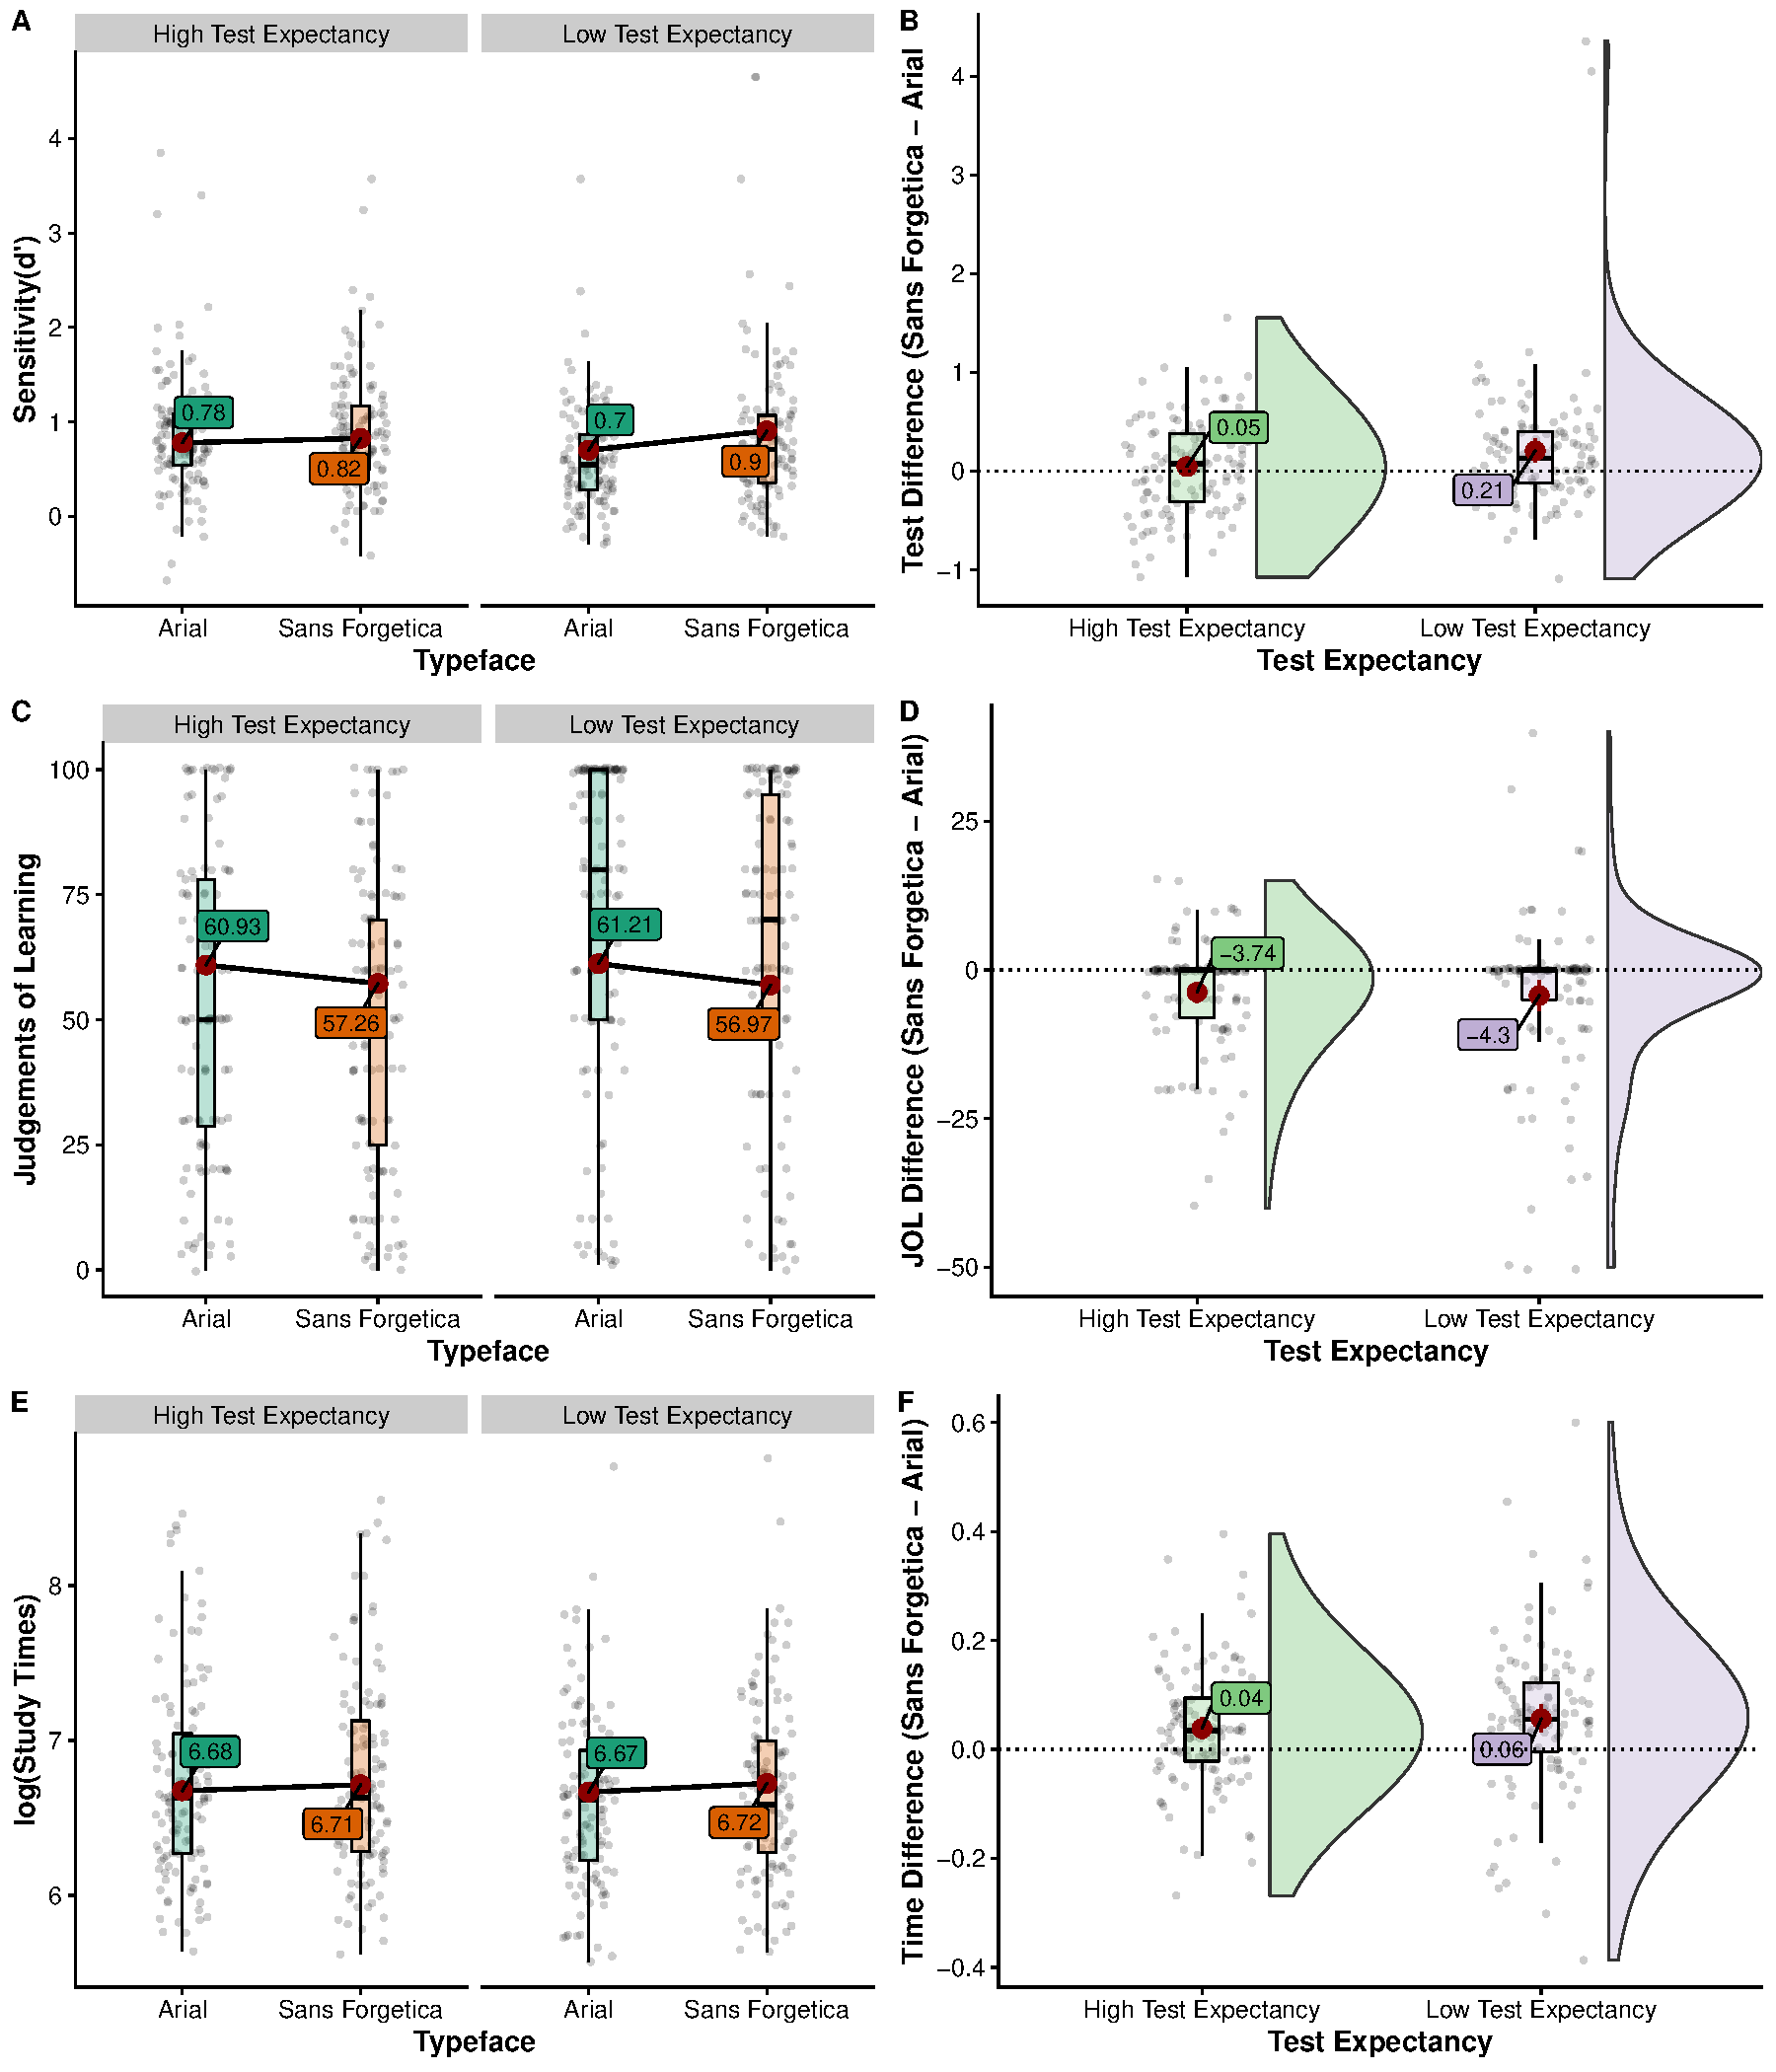
\includegraphics{Testing_Expectancy_SF_files/figure-latex/unnamed-chunk-19-1.pdf}

\hypertarget{general-discussion}{%
\section{General discussion}\label{general-discussion}}

Herein we have shown a boundary condition for the Sans Forgetica effect: testing expectancy. To summarize our findings, In Experiment 1 using a a recognition memory Sans Forgetica exerted a positive effect on memory when Partiicoanrs were not told about upcoming memory test. In experiment 21 Similar to other perceptual disfluency manipulations (masking, handwritten cursive) sans forgetica seemed to be o jefgive

Contrary to Experiments 1-3, when testing expectancy was low, we observed better memory for materials in Sans Forgetica. This provides a potential boundary condition for the Sans Forgetica effect. That is, when testing expectancy is high (e.g., Experiments 1-3) we do not see a Sans Forgetica effect. However, we do when testing expectancy is low. This might offer a potential explanation for why there is mixed evidence on the effectiveness of Sans Forgetica to enhance memory (See Eskenazi \& Nix, 2020). The results herein might explain why they did find a positive effect for Sans Forgetica in a subset of their participants. Despite this, given the small effect size and the fact that studying is almost always done intentionally, their is really no evidence that it should be used as a study tool.

RTs (one possible is optimal study hypothesis switching from harder stimuli to stumuli they know). JOLs would contradict this.

\newpage

\hypertarget{references}{%
\section{References}\label{references}}

\begingroup
\setlength{\parindent}{-0.5in}
\setlength{\leftskip}{0.5in}

\hypertarget{refs}{}
\leavevmode\hypertarget{ref-Balota2007}{}%
Balota, D. A., Yap, M. J., Cortese, M. J., Hutchison, K. A., Kessler, B., Loftis, B., \ldots{} Treiman, R. (2007). The english lexicon project. Springer New York LLC. \url{https://doi.org/10.3758/BF03193014}

\leavevmode\hypertarget{ref-Bjork2011}{}%
Bjork, E. L., \& Bjork, R. A. (2011). Making things hard on yourself, but in a good way: Creating desirable difficulties to enhance learning. In \emph{Psychology and the real world: Essays illustrating fundamental contributions to society.} (pp. 56--64). New York, NY, US: Worth Publishers.

\leavevmode\hypertarget{ref-Champely2020}{}%
Champely, S. (2020). \emph{Pwr: Basic functions for power analysis}. Retrieved from \url{https://CRAN.R-project.org/package=pwr}

\leavevmode\hypertarget{ref-Eitel2016}{}%
Eitel, A., \& Kühl, T. (2016). Effects of disfluency and test expectancy on learning with text. \emph{Metacognition and Learning}, \emph{11}(1), 107--121. \url{https://doi.org/10.1007/s11409-015-9145-3}

\leavevmode\hypertarget{ref-Eskenazi2020}{}%
Eskenazi, M. A., \& Nix, B. (2020). Individual Differences in the Desirable Difficulty Effect During Lexical Acquisition. \emph{Journal of Experimental Psychology: Learning Memory and Cognition}. \url{https://doi.org/10.1037/xlm0000809}

\leavevmode\hypertarget{ref-Geller2020}{}%
Geller, J., Davis, S. D., \& Peterson, D. J. (2020). Sans Forgetica is not desirable for learning. \emph{Memory}. \url{https://doi.org/10.1080/09658211.2020.1797096}

\leavevmode\hypertarget{ref-cogsci18-Geller}{}%
Geller, J., \& Still, M. L. (2018). Testing expectancy, but not judgements of learning, moderate the disfluency effect. In J. Z. Chuck Kalish Martina Rau \& T. Rogers (Eds.), \emph{CogSci 2018} (pp. 1705--1710).

\leavevmode\hypertarget{ref-Geller2018}{}%
Geller, J., Still, M. L., Dark, V. J., \& Carpenter, S. K. (2018). Would disfluency by any other name still be disfluent? Examining the disfluency effect with cursive handwriting. \emph{Memory and Cognition}, \emph{46}(7), 1109--1126. \url{https://doi.org/10.3758/s13421-018-0824-6}

\leavevmode\hypertarget{ref-Macmillan2005}{}%
Macmillan, N. A., \& Creelman, C. D. (2005). \emph{Detection theory: A user's guide, 2nd ed.} (pp. xix, 492--xix, 492). Mahwah, NJ, US: Lawrence Erlbaum Associates Publishers.

\leavevmode\hypertarget{ref-Morey2018}{}%
Morey, R. D., \& Rouder, J. N. (2018). \emph{BayesFactor: Computation of bayes factors for common designs}. Retrieved from \url{https://CRAN.R-project.org/package=BayesFactor}

\leavevmode\hypertarget{ref-Sagan1980}{}%
Sagan, C. (1980). \emph{Broca's brain: Reflections on the romance of science}. Retrieved from \url{https://books.google.com/books?hl=en\%7B/\&\%7Dlr=\%7B/\&\%7Did=GlXPqexwO28C\%7B/\&\%7Doi=fnd\%7B/\&\%7Dpg=PR4\%7B/\&\%7Dots=65nePfKWk5\%7B/\&\%7Dsig=CTTgqKJLaozsFvFqBYjBd\%7B/_\%7DEOkxE}

\leavevmode\hypertarget{ref-Singmann2020}{}%
Singmann, H., Bolker, B., Westfall, J., Aust, F., \& Ben-Shachar, M. S. (2020). \emph{Afex: Analysis of factorial experiments}. Retrieved from \url{https://CRAN.R-project.org/package=afex}

\leavevmode\hypertarget{ref-Sotola2020}{}%
Sotola, L. K., \& Crede, M. (2020). Regarding Class Quizzes: a Meta-analytic Synthesis of Studies on the Relationship Between Frequent Low-Stakes Testing and Class Performance. \emph{Educational Psychology Review}, 1--20. \url{https://doi.org/10.1007/s10648-020-09563-9}

\leavevmode\hypertarget{ref-Taylor2020}{}%
Taylor, A., Sanson, M., Burnell, R., Wade, K. A., \& Garry, M. (2020). Disfluent difficulties are not desirable difficulties: the (lack of) effect of Sans Forgetica on memory. \emph{Memory}, 1--8. \url{https://doi.org/10.1080/09658211.2020.1758726}

\endgroup


\end{document}
